%\documentstyle[epsf,twocolumn]{jarticle}       %LaTeX2e仕様
\documentclass[twocolumn]{jarticle}     %pLaTeX2e仕様(platex.exeの場合)
% \documentclass[onecolumn]{ujarticle}   %pLaTeX2e仕様(uplatex.exeの場合)
%%%%%%%%%%%%%%%%%%%%%%%%%%%%%%%%%%%%%%%%%%%%%%%%%%%%%%%%%%%%%%
%%
%%  基本バージョン
%%
%%%%%%%%%%%%%%%%%%%%%%%%%%%%%%%%%%%%%%%%%%%%%%%%%%%%%%%%%%%%%%%%
\setlength{\topmargin}{-45pt}
%\setlength{\oddsidemargin}{0cm}
\setlength{\oddsidemargin}{-7.5mm}
%\setlength{\evensidemargin}{0cm}
\setlength{\textheight}{24.1cm}
%setlength{\textheight}{25cm}
\setlength{\textwidth}{17.4cm}
%\setlength{\textwidth}{172mm}
\setlength{\columnsep}{11mm}

%\kanjiskip=.07zw plus.5pt minus.5pt


% 【節が変わるごとに (1.1)(1.2) … (2.1)(2.2) と数式番号をつけるとき】
%\makeatletter
%\renewcommand{\theequation}{%
%\thesection.\arabic{equation}} %\@addtoreset{equation}{section}
%\makeatother

%\renewcommand{\arraystretch}{0.95} 行間の設定
%%%%%%%%%%%%%%%%%%%%%%%%%%%%%%%%%%%%%%%%%%%%%%%%%%%%%%%%
%\usepackage{graphicx}   %pLaTeX2e仕様(\documentstyle ->\documentclass)
\usepackage[dvipdfmx]{graphicx}
\usepackage{subcaption}
\usepackage{multirow}
\usepackage{amsmath}
\usepackage{url}
\usepackage{ulem}
\usepackage{algorithm}
\usepackage{algorithmic}
\usepackage{listings} %,jlisting} %日本語のコメントアウトをする場合jlistingが必要
%ここからソースコードの表示に関する設定
\lstset{
  basicstyle={\ttfamily},
  identifierstyle={\small},
  commentstyle={\smallitshape},
  keywordstyle={\small\bfseries},
  ndkeywordstyle={\small},
  stringstyle={\small\ttfamily},
  frame={tb},
  breaklines=true,
  columns=[l]{fullflexible},
  numbers=left,
  xrightmargin=0zw,
  xleftmargin=3zw,
  numberstyle={\scriptsize},
  stepnumber=1,
  numbersep=1zw,
  lineskip=-0.5ex
}
%%%%%%%%%%%%%%%%%%%%%%%%%%%%%%%%%%%%%%%%%%%%%%%%%%%%%%%%
\begin{document}

	%bibtex用の設定
	%\bibliographystyle{ujarticle}

	\twocolumn[
		\noindent
		\hspace{1em}
		2020 年 5 月 22 日
		ゼミ資料
		\hfill
		B4 杉山 竜弥
		\vspace{2mm}

		\hrule
		\begin{center}
			{\Large \bf 進捗報告}
		\end{center}
		\hrule
		\vspace{9mm}
	]

	% ‚ここから 文章 Start!
\section{今週やったこと}
\begin{itemize}
	\item {2クラスと4クラスの分類}
\end{itemize}

\section{問題設定}
% 何を入力として何を出力とするかを明確に定義

 データを正解と不正解に分割して学習する以下のアルゴリズム1を考える.

	\begin{algorithm}
		\caption{Swap two datasets}
		\label{alg1}
		\begin{enumerate}{ % itemize, enumerate, description
			\item{データ 2N 抜き出す}
			\item{そのデータを ランダムに N(A) と N(B)に分ける.}
			\item{X : A → train, B → test で学習}
			\item{Y : B → train, A → test で学習}
			\item{3.と4.で test でミスしたデータを調べる}
			\item{A をテストとしたとき失敗したデータと B をテストとしたとき成功したデータを入れ替える.ただし, 同じクラスのデータ同士.}
			\item{モデルを初期化して, 3.に戻る.}
		}\end{enumerate}
			% \begin{algorithmic}
			% \end{algorithmic}
	\end{algorithm}

	データのクラスが同じもの同士を入れ替えることで, データセットのクラス比が変化しないようにした.
  学習中に入れ替えるのではなく, 学習が終わった後入れ替え, 再び学習する際にモデルのパラメータは初期化した.


\section{実験}

	\begin{table}[tb]
		\begin{center}
			\caption{実験の設定}
			\begin{tabular}{|c|c|} \hline
				dataset & cifar10 \\
				data N & 5,000 / model \\ \hline
				task & 2 or 4クラス識別 \\
				input & image(3x32x32) \\
				output & class(2 or 4) \\ \hline
				model & CNN(16層) \\
				optim & SDG (lr=0.001, moment=0.9) \\
				loss & Cross Entropy Loss \\ \hline
				batch size & 16 \\
				epoch & 20 \\ \hline
        swap & 15 \\ \hline
			\end{tabular}
			\label{tab:setting}
		\end{center}
	\end{table}

今回はcifar10に含まれる10クラスの内, 2クラスの場合と4クラスの場合の簡単な分類タスクを用意して, 前回の10クラスに近い条件で同様の実験を行った.

\subsection{結果}

前回よりもクラス数が減ったため, ベースラインも上昇した. それと共に図\ref{fig:accuracy}のように高い精度が実現できた. 単にCNNの出力層を変えただけであるため, 実行時間はほとんど変化なく90分程であった. epoch数を増やすことはできなかったが20 epoch時点の精度で十分であると判断した.

前回10クラスで精度は2モデルとも似た推移をとったが, 2クラス, 4クラス共に手順4のモデルの精度が高い性能を示した. これはアルゴリズムから予想通りで, 前回と比べ十分に精度が出る問題に設定したため, 2つのデータセット間の入れ替えでテスト結果が強く反映されたと考えられる.

% 手順6で入れ替えるデータ数は, 失敗データと成功データを交換するので精度50 \%のとき最も頻繁に入れ替えされる.

図\ref{fig:swapclass}では手順6でのデータ入れ替え数を示した. 入れ替えの多くが鳥(bird)クラスに占められており, 逆に自動車(automobile)クラスは入れ替えが少なかった.

さらに入れ替えを調べるため, 図\ref{fig:swaptimes}には入れ替え頻度分布を示した. 実験では15回の交換を行ったため, あるデータが頻繁に入れ替えられたときグラフでは15回に近い値をとる. 自動車は交換されたものはほとんどが1回なのに対し, 鳥は何度も入れ替えられていることが分かった. 自動車が簡単な分類であるため, モデルのテスト結果が変化せず, 入れ替えが起こりにくかったと思われる.

\begin{figure}[tb]
	\begin{center}
		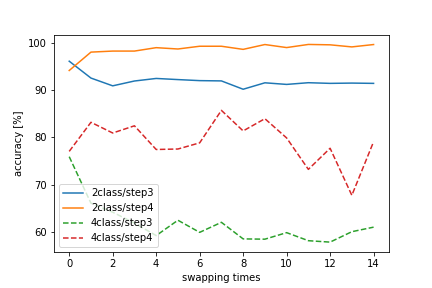
\includegraphics[clip,width=8.5cm]{accuracy.png}
		\caption{学習後モデルのテストの精度 
		実線が2クラス分類,
    点線が4クラス分類}
		\label{fig:accuracy}
	\end{center}
\end{figure}
\begin{figure*}[tb]
	\begin{center}
		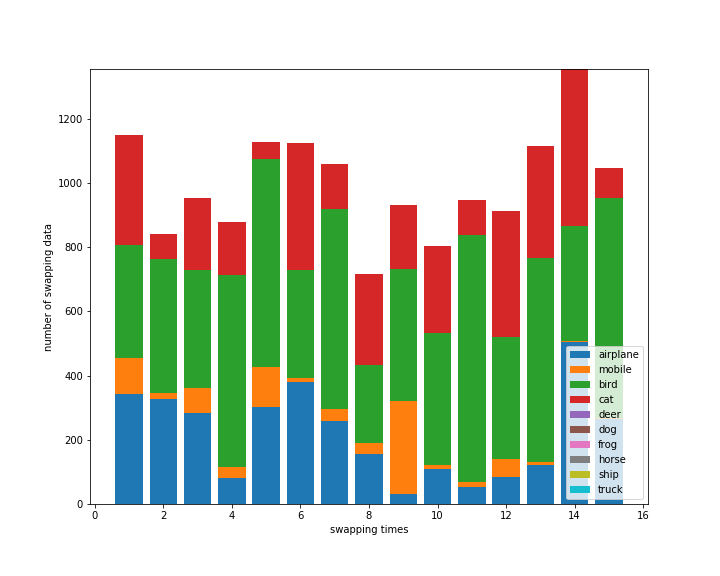
\includegraphics[clip,width=13cm]{swapclass4.png}
		\caption{4クラス分類でのデータ入れ替え数 }
		\label{fig:swapclass}
	\end{center}
\end{figure*}
\begin{figure*}[tb]
	\begin{center}
		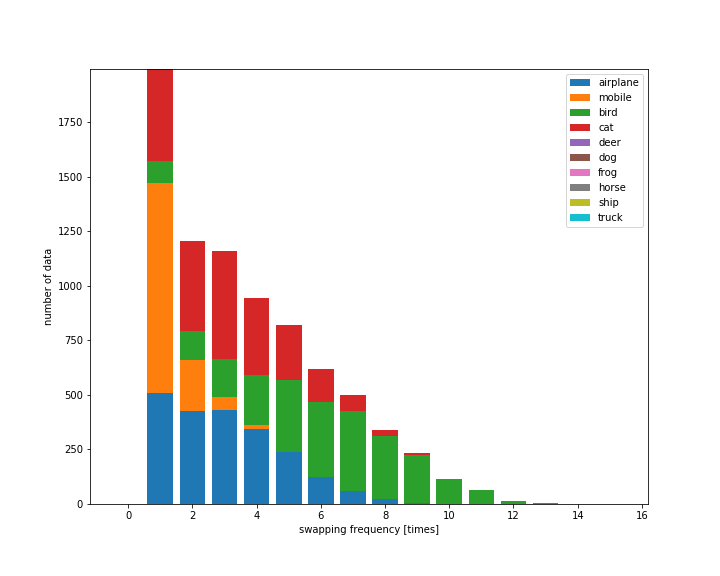
\includegraphics[clip,width=13cm]{swaptimes4.png}
		\caption{4クラス分類でのデータの入れ替え頻度分布 
		% あるデータが何度も入れ替えられるとX軸方向にいく
    (0 $\leq$ 同じデータが入れ替えられた度数 $\leq$ 15)
    }
		\label{fig:swaptimes}
	\end{center}
\end{figure*}

\section{考察}
% 精度が出ない,とかだけではなく自分なりの考察を示す
前回とほとんど変化のないコードで大きく異なる結果となったのは, 問題の難しさに対して前回のモデルが十分に機能していなかったことが考えられる. 問題を簡単にすることによって, データセットの特性が顕著になったと言える.

頻度分析をすることで交換されるデータの流れやクラスごとの違いが分かった. またテスト精度をクラスごとに分けることで, 鳥クラスが何度も入れ替えられた原因を探りたい.

\section{今後の予定}
% なんとなくなんかの勉強をするとかではなく具体的に
\begin{itemize}
	\item {精度を高めるためのモデルの調整}
\end{itemize}

\section{ソースコード}
% 埋め込みでもGitでもいいので参照できるように

% \begin{lstlisting}[caption=cnn,label=model_cnn]
% code
% \end{lstlisting}


% 参考文献リスト
\bibliographystyle{unsrt}
\bibliography{ref}
\end{document}
